\documentclass[../main.tex]{subfiles}
\begin{document}
	\chapter{Machine Learning} \label{ch:machine}
	

	\section{Machine Learning Basics}
	\noindent 
	
	\noindent  \textit{Machine Learning} focuses on the development of algorithms and models that enable computers to learn from data with the aim of making predictions without being explicitly programmed. \\ \\ 
	The machine learning model is built using one or more input variables which are also called \textbf{predictors} or independent variables. The output of this model is the \textbf{response} or dependent variable which we want to predict. Machine learning is about learning an approximate function that can be used to predict the value of response variable.\\ \\
	We can think about learning as the way we understand it as a human. We can classify a learning problem based on the degree of feedback. Machine learning models fall into three primary categories:
	\begin{itemize}
		\item Supervised learning, where we have immediate feedback.
		\item Reinforcement learning, where we have indirect feedback. For example when we are playing the game of chess.
		\item Unsupervised learning, where we have non-feedback signal. For example, deducing which dog belongs to each owner.
	\end{itemize}
	Machine learning models simplify reality for the purposes of understanding or prediction. This prediction can be either a numerical prediction or a classification prediction. A number of machine learning algorithms are commonly used, for example to name a few: linear regression, logistic regression, decision trees, random forests...
	\\ \\ \\ \\ \\ 
	
	\subsection{Motivation }
	\noindent In order to motivate our study of machine learning, we are going to present some examples.  
	
	\begin{xmpl}
	
	Let us consider the following hypothetical scenario.  Imagine that we are the Data Scientist of a big football club. The club needs a new main striker for the next season and we are tasked with evaluating each candidate and decide whether to sign them or not. We have loads of data from each player. \\ 
	
	\begin{tabular}{ll}
		\toprule
		\textbf{Player Attributes Last Season:}  \\ 
		\midrule
		Age & 21 \\
		Matches Played & 38 \\
		Goals& 14\\
		Assists & 11\\
		Expected goals & 10.56 \\
		Shots on target& 32 \\
		... & ... \\
		\bottomrule
	\end{tabular} 
	\\ 
	\begin{itemize}
		\item Input: \textbf{$x_c=(x_{c_1},...,x_{c_d})$}  "attributes of the player". 
		\item Output:  
		\[
		y = \begin{cases}
			\text{sign} \\
			\text{not sign}& \\
		\end{cases}
		\]
		
		\item Target funtion: $f$  "ideal player signing formula".
		\item The dataset $\{(x_1, y_1), (x_2, y_2), ..., (x_n, y_n)\}$ consists of historical records of strikers, where $x_i$ represents the player's attributes and $y_i$ indicates the classification of whether they were signed or not.
	\end{itemize}
	
	\noindent We are looking for the function $f$ such that $f(x_c)=y$.
	\end{xmpl}
	\noindent 
	An important aspect of machine learning is that \textit{many supervised learning tasks are about function learning.} In general, a fundamental problem in machine learning can be defined as follows: given a dataset of the form $\{(x_i,y_i)\}^m_{i=1} \subset \mathbb{R}^n \times \mathbb{R}$, the goal is to find a model $f$ that accurately predicts the output $y_i$ for a given input $x_i$.
	
	\begin{xmpl}
		\noindent An example of a supervised learning task is digit recognition. The objective is to identify handwritten digits (0-9) based on input images. In this task, we aim to learn a probability distribution function denoted as $f$, which maps a set of pixel values ranging from 0 (black) to 255 (white), representing a 28x28 image, to a probability distribution over the digits 0 to 9. In practice, we often learn the function 
		$$f: \{0,...,255\}^{28 \times 28} \longrightarrow \mathbb{R}^{10}$$
		where big values represents that is very likely and small very unlikely. 
	\end{xmpl}
	\begin{xmpl} Example of a classification problem. We want to classify if an image is a dog or not a dog. We would like to produce a value which is correlated with the probability of this image being a dog or not a dog.  We can approach the problem in the following way. We want to find a function that takes very high values when dog-image and very low val ues when non dog images and takes the value 0 when its uncertain. That function is
		$$d: \mathbb{R}^{\# \text{pixels in image}} \rightarrow \mathbb{R}. $$
		
		\noindent This is what we mean by many problems can be recast as function learning. Note that there is not a god-given reason why this function should exist. We know that certain points in space, and they have certain values associated to them, but we dont know that there is some function. 
	\end{xmpl}

	
	\subsection{Linear Regression}
	\noindent A linear regression algorithm is used to predict numerical values, based on a linear relationship between different values. A simple linear model is defined by the following equation:
	$$ y_i=  w_0 +w_1 x_i +\epsilon_i  $$
	\noindent where $ i = 1, ..., n$.  \\ \\ 
	Note that $y$ is the dependent variable (response), $x$ is the independent variable (predictor), $w_0$ is the intercept, $w_1$ is the slope coefficient and $\epsilon$ is the error term or the residual. \\ 
	\begin{figure}[h]
		\centering
		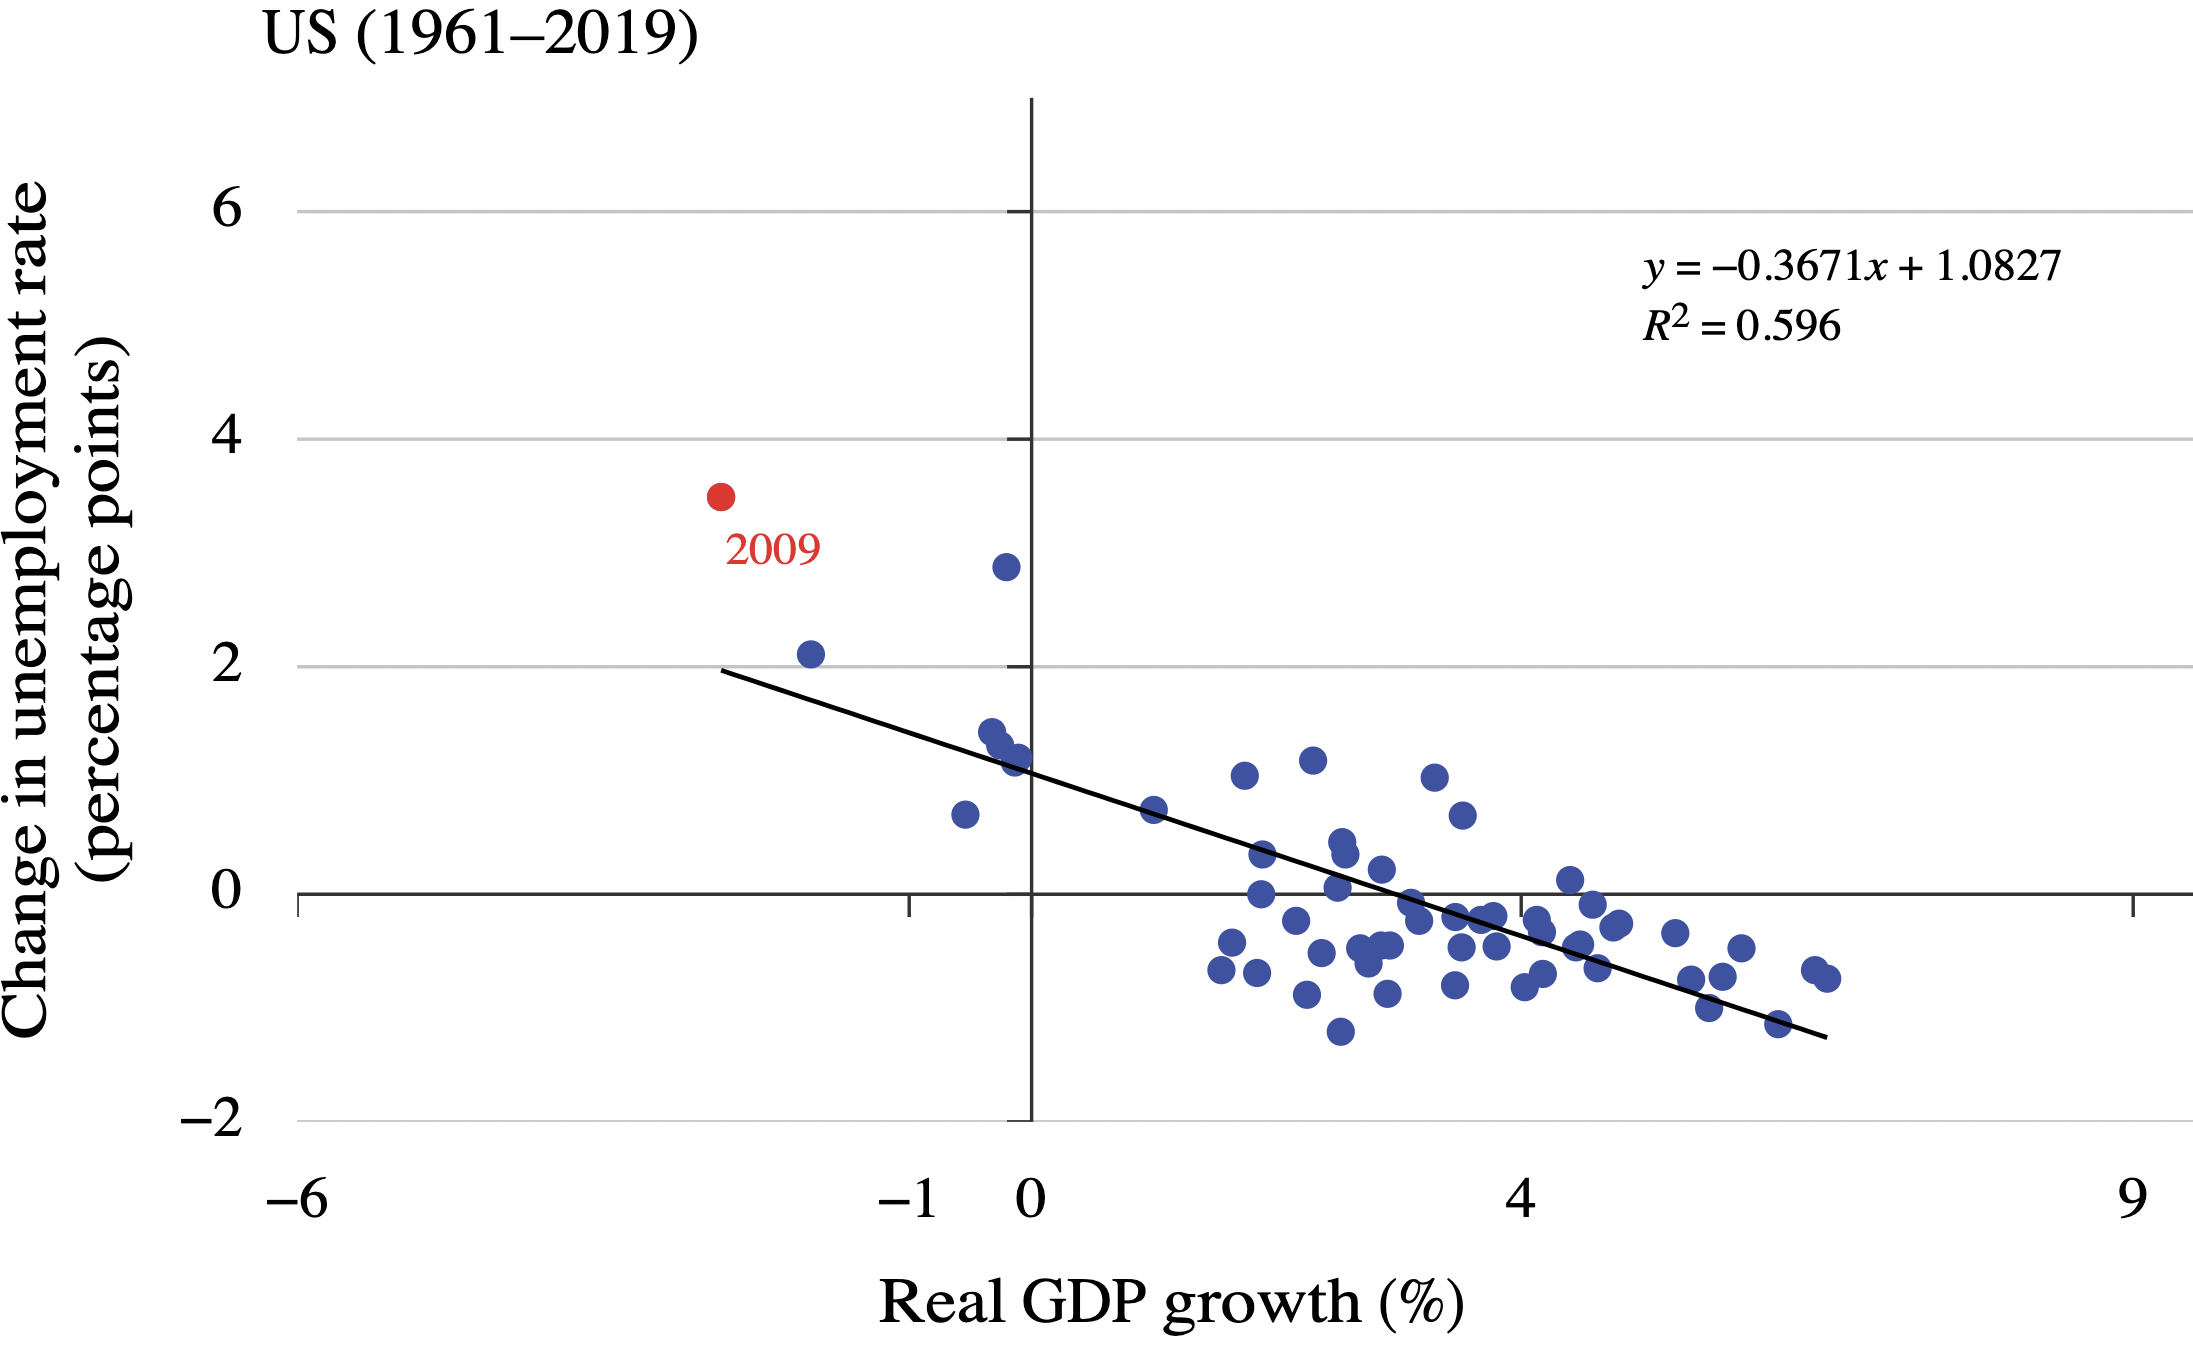
\includegraphics[width=0.6\linewidth]{imgs/gdp.png}
		 \caption{\small $y$ response variable: unemployment rate , $x$ predictor: GDP growth.} 
	\end{figure} \mbox{} \par
\vspace{\baselineskip} 
\noindent We can add additional $p$ predictors to a simple linear model, transforming it into a multivariate linear model, which we define as follows:

$$y_i = w_0 + w_1x_{1i} + \ldots + w_px_{pi} + \epsilon_i. $$

\noindent More commonly, the multivariate linear regression equation is expressed in matrix form as: $y = w^T x + \theta $.



\subsection{Logistic Regression}
\noindent Logistic regression is a model for predicting the probability that a binary response is 1.  It is suitable for classification tasks, as well as for prediction of probabilities.  From a statistical perspective, it is defined by assuming that the distribution of the binary response variable, $y$, given the features, $x$, follows a Bernoulli
distribution with success probability $p$. 

\[P(y = 1 | X = x) = p 
\qquad  \text{and}
\qquad
P(y = 0 | X = x) = 1-p. \]
We need to define the concept of sigmoid function that will be important along the work. A \textit{sigmoid function} is a mathematical function that maps input values to a range between 0 and 1. We consider the following sigmoid function, the logit inverse function:

\[
\text{logit}: (0,1) \to \mathbb{R}
\quad \text{and is expressed as:} \quad
\text{logit}(x) = \log\left(\frac{x}{x-1}\right)
\]


\[
\text{logit}^{-1}: \mathbb{R} \to (0,1)
\quad \text{and is expressed as:} \quad
\text{logit}^{-1}(x) = \frac{e^x}{1+e^x}
\]

\noindent The linear predictor, $ w^T x +\theta$, fluctuates between $(-\infty,\infty)$ where $x$ represents all predictors in the model. To address this difference in scale, the outcome variable is transformed using the logit function. The logistic regression model assumes a linear (affine) relationship between the feature vector $x_i$ and the log odds of $p$. Namely,
$$\text{logit}(p) = w^T x +\theta$$

\noindent The logistic model can be alternatively expressed using the inverse logit function:

\[
P(y = 1 | X=x) = \text{logit}^{-1}(w^T x +\theta)
\]




\section{Multilayer Feedforward Networks}
	
	 
	 \noindent \textit{Artificial Neural Networks} (ANN) are the quintessential deep learning models, especially \textit{multilayer feedforward networks}. They are widely used for nonlinear function approximation. The goal of an artificial neural network is to approximate some function $f^*$. For example, for a classifier, $y = f^*(x)$ maps an input $x$ to a category $y$.  \\ \\ 
	 %A feedforward network defines a mapping $y = f(x;\theta)$ and learns the value of the parameters $\theta$ that result in the best function approximation. \\ \\ 
	 \noindent The term \textit{neural} refers  to the fact that this model was originally inspired by how biological neurons process information. \\ \\ 
	 \noindent The term \textit{feedforward} indicates the direction of information flow within the network, moving only forward in contraposition to backwards. Each layer processes the input data and passes its output to the next layer, creating a sequence of transformations until the final output is produced. \\ \\
	 \noindent The term \textit{network} refers to the interconnected structure of artificial neurons. A multilayer network consists of multiple layers, including an input layer, one or more hidden layers, and an output layer. \\ \\ %The neurons within each layer are connected to the neurons in the subsequent layer, forming a network of connections. The connections between neurons are represented by weights, which determine the strength and influence of each neuron's output on the inputs of the subsequent layer. \\ \\ 
	 \noindent The architecture of the network entails determining its \textit{depth}, \textit{width}, and \textit{activation functions} used. Depth is the number of hidden layers. Width is the number of units (nodes) on each hidden layer. The \textit{activation function} defines how the weighted sum of the input is transformed into an output from a node in a layer of the network. Because the activation function plays a crucial role in our work, further details regarding its importance will be provided in the next section.
	 
	 
	 %they are composed of interconnected processing units called artificial neurons, which are organized in layers and are capable of learning and generalizing from data.	
	 \section{Architecture of a Multilayer Feedforward Network}
	 \subsection{Artificial neuron}
	 \noindent The equation
	  \begin{equation}
	  	y=\sigma(w^Tx + \theta) \tag{2}
	  	\label{eq:sig}
	  \end{equation}
  
   \noindent represents what we may call a \textit{single layer of a deep learning model}, also called an \textit{artificial neuron}.  Observe that the artificial neuron is composed of an affine transformation $ z=w^Tx + \theta$ followed by a (generally) non-linear transformation $\sigma(z)$. \\ \\ In more detail, $x \in \mathbb{R}^n$ is the input vector and represents a set of $n$ features or predictors, $w\in  \mathbb{R}^n$ is the weights vector where each element of the weights vector $w_i$ corresponds to the importance assigned to the corresponding input feature $x_i$. $\theta$ is the bias and $\sigma$ is the activation function. The result variable is a scalar output $y \in \mathbb{R}$. 
 
   
   \begin{figure}[h]
   	\centering
   	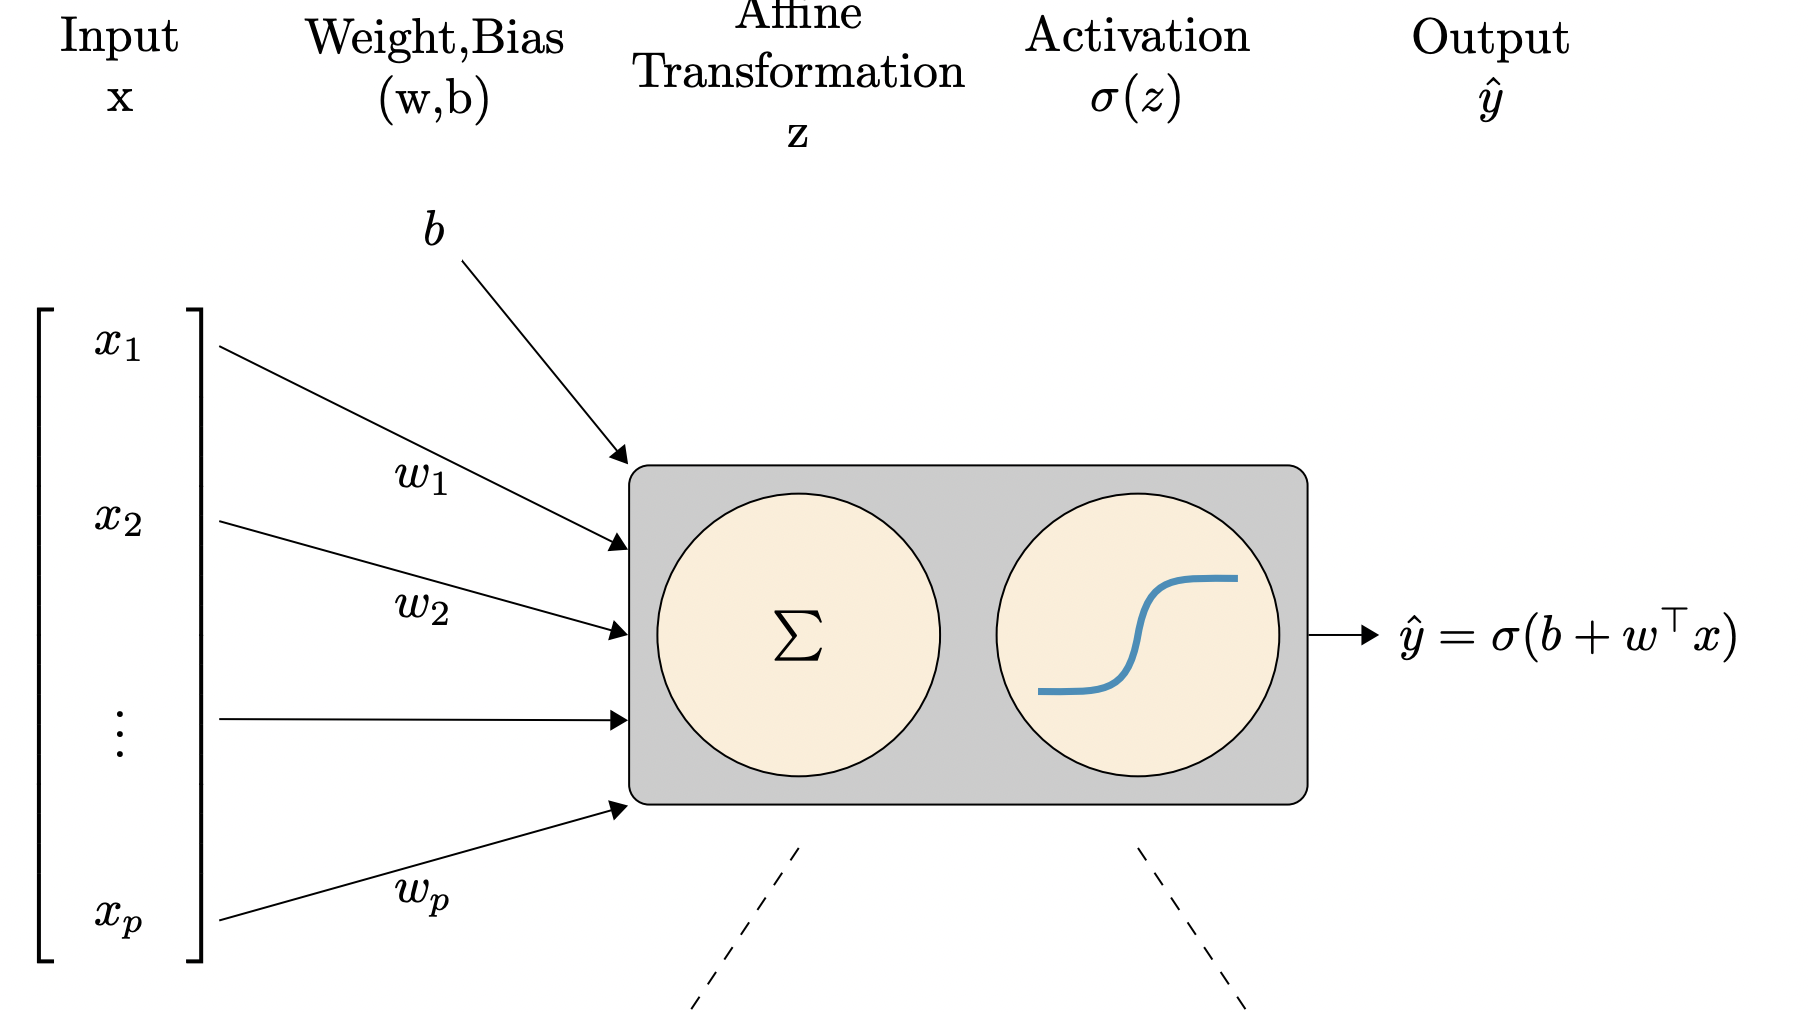
\includegraphics[width=0.8\linewidth]{imgs/neu}
   	\caption{\small Artificial neuron} 
   \end{figure} \mbox{} \par
   
  
 \subsection{Activation Function}
 
 
 \noindent The introduction of the activation function in ANN was inspired by biological neural networks whose purpose is to decide whether a particular neuron fires or not. The simple addition of such function can tremendously help the network to exploit more, thereby learning faster. There are various activation functions proposed in the literature, and it is difficult to find the optimal activation function that can tackle any problem. \\ \\ 
	 	\noindent Note that a logistic regression is an artificial neuron where the activation function  $\sigma$ is $\text{logit}^{-1}$. Two widely popular activation functions are the Hyperbolic Tangent and Rectified Linear Unit (ReLU):
	 	
	
	
	\[
	\text{Hyperbolic Tangent (\text{tanh}): } \mathbb{R} \to (-1,1)
	\]
	
	

	 and 
	  \[
	 \text{ReLU}: \mathbb{R} \to (0,\infty)
	 \quad \text{and is expressed as:} \quad
	 \text{ReLU}(x) = \max(0,x)
	 \]
	 
	 
	 
	 \begin{figure}[h]
	 	\centering
	 	
	 	\begin{tikzpicture}
	 		\begin{axis}[
	 			xmin=-5, xmax=5,
	 			ymin=-0.5, ymax=1.5,
	 			axis lines=middle,
	 			xlabel=,
	 			ylabel=,
	 			xtick=\empty,
	 			ytick={0,1},
	 			samples=100,
	 			smooth,
	 			scale=0.5
	 			]
	 			\addplot[blue, thick, domain=-5:5] {1/(1+exp(-x))};
	 		\end{axis}
	 	\end{tikzpicture}
	 	\hspace{1cm}
	 	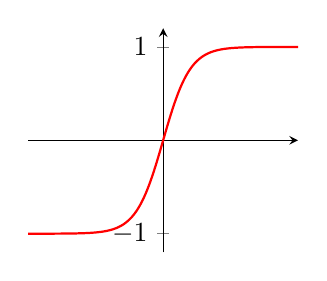
\begin{tikzpicture}
	 		\begin{axis}[
	 			xmin=-5, xmax=5,
	 			ymin=-1.2, ymax=1.2,
	 			axis lines=middle,
	 			xlabel=,
	 			ylabel=,
	 			xtick=\empty,
	 			ytick={-1,1},
	 			samples=100,
	 			smooth,
	 			scale=0.5
	 			]
	 			\addplot[red, thick, domain=-5:5] {tanh(x)};
	 		\end{axis}
	 	\end{tikzpicture}
	 	\hspace{1cm}
	 	\begin{tikzpicture}
	 		\begin{axis}[
	 			xmin=-5, xmax=5,
	 			ymin=-0.5, ymax=5,
	 			axis lines=middle,
	 			xlabel=,
	 			ylabel=,
	 			xtick=\empty,
	 			ytick=\empty,
	 			samples=100,
	 			smooth,
	 			scale=0.5
	 			]
	 			\addplot[green, thick, domain=0:5] {max(0,x)};
	 			\addplot[green, thick, domain=-5:0] {0};
	 		\end{axis}
	 	\end{tikzpicture}
	 	
	 	\caption{Graphs of the sigmoid, hyperbolic tangent, and ReLU functions.}
	 \end{figure}
	 	
	 \subsection{Definition}
	 \noindent  We now get into more details on the precise definition of a deep neural network, which is after all a purely mathematical object. 
	 \begin{definition} A \textit{multilayer feedforward network} is the function
	 	$$f(x)=\sum_{j=1}^k \beta_j \cdot \sigma(w_j \cdot x - \theta_j)$$
	 	where $x \in \mathbb{R}^n$ is the input vector, $k \in \mathbb{N}$ is the number of processing units in the hidden layer, $w_j \in \mathbb{R}^n$ is the weight vector that connects the input to processing unit $j$ in the hidden layer, $\sigma : \mathbb{R} \rightarrow \mathbb{R}$ is an activation function, $\theta_j \in \mathbb{R}$ is the threshold (or bias) associated with processing unit $j$ in the hidden layer, and $\beta_j \in \mathbb{R}$ is the weight that connects the processing unit $j$ in the hidden layer to the output of the network.
	 	
	 	
	 \end{definition}
	 
	 \noindent Let $N_{w}$ be the family of all functions that can be describe with a given network architecture.  If we can show that $N_{w}$ is dense in $C(\mathbb{R}^n)$, we can conclude that for every continuous function $g \in C(\mathbb{R}^n) $ and each compact set $K \subset \mathbb{R}^n$, there is a function $f \in N_{w}$ such that $f$ is a good approximation to $g$ on K. \\ \\
	 \noindent The guiding question of the present work is: under which necessary and sufficient conditions on $\sigma$ will the family of networks $N_w$ be capable of approximating to any desired accuracy any given continuous function?
	 
	 	\begin{figure}[h]
	 	\centering
	 	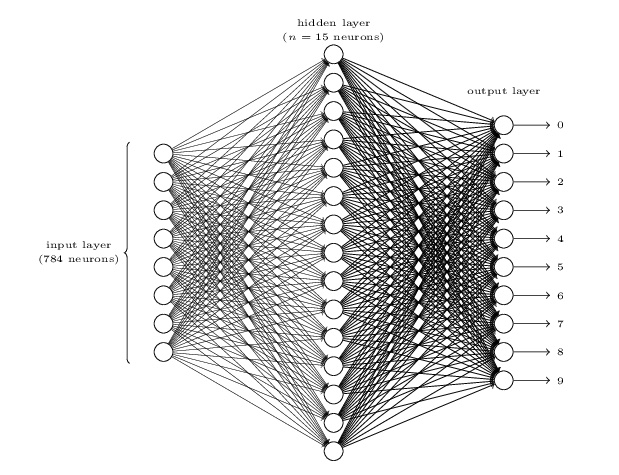
\includegraphics[width=0.9\linewidth]{imgs/neural-network-2.jpg}
	 	\caption{\small Multilayer neural network} 
	 \end{figure} \mbox{} \par
	
\end{document}